% This must be in the first 5 lines to tell arXiv to use pdfLaTeX, which is strongly recommended.
\pdfoutput=1

\documentclass[11pt]{article}

% "review" adds margin line numbers; this is the final version, so it is removed.
\usepackage{ACL2023}

% Standard package includes
\usepackage{times}
\usepackage{latexsym}
\usepackage[capitalize]{cleveref}

\usepackage[T1]{fontenc}
\usepackage[utf8]{inputenc}
\usepackage{microtype}
\usepackage{inconsolata}
\usepackage{graphicx}
\usepackage{amsmath}

\title{Why Separable Subjects Still Fail to Link:\\
A Streaming Journal over Knesset Committee Protocols}

\author{Tomer Morad \\ \texttt{tomermorad1@gmail.com} \And
  Or Israeli \\ \texttt{or.israeli2@mail.huji.ac.il} \And
  Yoel Marko \\ \texttt{yoel.marcu2003@mail.huji.ac.il}}

\begin{document}
\maketitle

\begin{abstract}
We build a longitudinal journal over a stream of Israeli Knesset Finance Committee
transcripts, coupling three tasks --- topic segmentation, \emph{streaming} cross-document
subject linking, and update summarization --- under an asymmetric cost model in which merging
two distinct matters is worse than splitting one. Our central result is negative and, we
argue, the most useful thing the project produced. On a manually annotated set of 523
segments, one fixed representation (\texttt{multilingual-e5-large}$+$ABTT) scores
$F_1{=}0.619$ judging subject identity over \emph{pairs}, and $F_1{=}0.125$ when the
\emph{same representation} makes the \emph{same decision} online against a growing journal.
The collapse is caused not by weak Hebrew embeddings but by the streaming decision structure,
where only $6.9\%$ of arrivals are true repeats. Under a matched streaming-honest protocol a
distinctiveness \emph{margin} rule raises $F_1$ $0.087{\to}0.190$, while every LLM verifier
stays $\le 0.111$. We further document two ways this benchmark rewards look-ahead.
\end{abstract}

\section{Introduction}

A parliamentary committee returns to the same matter --- a bill, a budget transfer, a
programme --- again and again over months, so reconstructing the history of any one matter
means reading dozens of unrelated transcripts. We produce that history automatically: an
index in which each entry is one underlying matter carrying a dated log of its progress.
The problem decomposes into three coupled tasks. \textbf{Segmentation} partitions each
protocol into subject spans; \textbf{streaming subject linking} decides, for each arriving
span, whether it continues an existing entry or opens a new one; and \textbf{log writing}
generates only the \emph{incremental} update to the matched entry.

\paragraph{How this is done today, and its limits.}
Task 2 is a variant of cross-document event coreference
\cite{cybulska2014sledgehammer,barhom2019revisiting}, but the standard setting is
\emph{offline}: a system sees the whole collection and clusters it globally. Ours is online
over a growing index, with no look-ahead and its own past errors persisting. Task 3 is
update summarization \cite{dang2008update} with retrieval augmentation \cite{lewis2020rag};
unlike query-conditioned RAG, faithfulness is defined relative to a \emph{chain of prior
summaries} rather than a source document, because the retrieved log records what has already
been written.

\paragraph{Asymmetric cost.}
Merging two distinct matters corrupts an entry permanently and silently; splitting one is
visible and repairable. We therefore report every operating point twice: at best $F_1$, and
at the \emph{anti-duplication} point where the false-merge rate (FMR) is held $\le 5\%$.

\paragraph{Contributions.}
We expected the bottleneck to be Hebrew representation quality; it is not. Our research
question became: \emph{why does near-ceiling subject separability fail to produce usable
streaming linking, and what closes the gap?} We contribute (i) a manual gold standard over
$211/213$ protocols; (ii) a quantification of the separability/decision gap with a base-rate
explanation; (iii) a matched ablation of the levers that close it, all structural rather
than representational; (iv) evidence that an LLM helps as an \emph{extractor} but not a
\emph{classifier}; and (v) two look-ahead leaks found in our own pipeline. Any index built
incrementally over a stream faces the same arithmetic, and our diagnosis predicts a better
encoder will not help.

\section{Data}
\label{sec:data}

We use 213 Hebrew transcripts of the 25th Knesset Finance Committee (2022-11-21 to
2023-10-26); each is one meeting, given as committee, ISO date and the full transcript.
Protocol-level subject markers yield 151 canonical topics after fuzzy variant merging, but
these describe the \emph{meeting}, not the spans inside it, so we manually segmented
$211/213$ protocols into subject spans labelled with the matter under discussion
(\cref{tab:data}).

Two properties dominate what follows. We deliberately did \emph{not} merge near-duplicate
labels across protocols --- under our cost rule an unmerged duplicate is a cheap false
split, whereas a wrong merge would corrupt the gold itself --- so recurrence counts are
conservative. And, decisively, repeats are \emph{rare}: 36 of 523 arrivals continue an
existing matter, a base rate of $6.9\%$.

\section{Methods}

\paragraph{Representation.}
Segments are embedded with \texttt{multilingual-e5-large} \cite{wang2024multilinguale5},
using discussion content only --- no headers, agendas, attendees or speaker names. Dense
encoders are severely anisotropic \cite{ethayarajh2019contextual}: here cross-topic cosine
averages ${\approx}0.95$, leaving a same/different gap of $0.007$--$0.066$. We apply
All-But-The-Top (ABTT) \cite{mu2018allbutthetop} --- centre, project out the top-$k$
principal directions, re-normalise --- and compare against TF-IDF and AlephBERT
\cite{seker2022alephbert}.

\paragraph{Two evaluation protocols.}
\textbf{Pairwise} scores all segment pairs and measures \emph{separability}, with oracle
access to the full set. \textbf{Streaming} presents segments chronologically and scores each
against the journal built so far --- the actual task.

\paragraph{Levers.}
An entry is represented either by its \emph{first span, frozen} or by the running
\emph{centroid} of its members; the rule is either a flat threshold
($\cos_{(1)} \ge \theta$) or a \emph{distinctiveness margin}
($\cos_{(1)} - \cos_{(2)} \ge \theta$). We vary one lever at a time, CPU-only, holding
transform, fitting protocol and growth model fixed.

\paragraph{LLM as verifier, LLM as extractor.}
Following retrieve-then-verify we shortlist by dense retrieval and ask an LLM to classify
\emph{same}/\emph{related}/\emph{new}, from a candidate snippet and from its \emph{full
accumulated timeline}. Separately we use it as an \emph{extractor} of stable fingerprints
(ministries, laws, programmes, request numbers), fusing identifier overlap additively with
the geometric margin. Models: \texttt{dictalm2} \cite{shmidman2024dictalm} and
\texttt{qwen2.5} at 3B/7B.

\paragraph{Streaming-honest fitting.}
ABTT and whitening estimate parameters \emph{from data}; fitting once over the whole matrix
uses segments that have not arrived. We refit at every step from the observed prefix, and
report batch and honest numbers side by side.

\vspace{-2pt}

\paragraph{Log writing.}
Each update is conditioned on the running journal built from the model's \emph{own} prior
generations, so faithfulness is chain-relative. Since predicted links are only
${\approx}13\%$ precise, evaluating through them would conflate two failures; we use
\textbf{gold chains} (22 matters, 58 entries), judged by \texttt{Qwen2.5-3B-Instruct} ---
neither generator --- for \emph{faithfulness} and \emph{novelty}.

\section{Results}

\paragraph{De-anisotropisation matters more than encoder choice.}
\cref{tab:repr} shows that removing a \emph{single} principal direction moves \texttt{e5}
from ARI $0.124$ to $0.657$ --- more than the entire spread across \texttt{e5}, TF-IDF and
AlephBERT. Before ABTT, TF-IDF beats every dense model: the discriminative signal is lexical
and the dense geometry is dominated by shared bureaucratic register. We fix
\texttt{e5}$+$ABTT-$k$1 throughout.

\paragraph{The separability/decision gap.}
\cref{tab:gap} and \cref{fig:gap} give the central result: a representation separating
same- from different-matter pairs at $F_1\,0.619$ collapses to $F_1\,0.125$ when the same
decision is made online. \textbf{The bottleneck is the streaming decision structure, not
representation quality.}

The cause is a base-rate effect. Only 36 of 523 arrivals are repeats, and each is compared
against a journal growing toward several hundred entries, so with $n$ candidates expected
false merges scale as $n\cdot\mathrm{FPR}$ while true positives stay at most one --- a
false-positive rate low enough to look excellent pairwise still floods the true matches.
Notably, \textbf{retrieval was never the bottleneck}: ranking places the correct entry in the
top 10 for \emph{all} 36 repeats (recall@1 $0.694$, @5 $0.944$, @10 $1.000$). The information
is in the shortlist; the \emph{decision} fails. \cref{tab:examples}(a) shows why: a segment
and its true continuation --- same ministry, same request number --- score $0.266$, while an
unrelated ministry's transfer scores $0.448$, shared administrative phrasing outweighing the
sparse identifying tokens.

\paragraph{What closes the gap.}
\label{sec:centroid}
\cref{tab:levers} varies one lever at a time with everything else fixed. The
\textbf{distinctiveness margin} is the decisive change: $F_1$ $0.087\to0.190$ and recall at
FMR$\le5\%$ from $0\%$ to $8.6\%$. It targets the failure mode in
\cref{tab:examples}(a) --- with families of near-identical templates, high absolute
similarity is uninformative while a large \emph{gap} is not.

Replacing the frozen first span with the running centroid is a large \emph{recall} fix: on
the batch-fit ABTT-$k$1 path it lifts recall $32\%\to89\%$ ($F_1$ $0.103\to0.107$), because
the streaming setting keeps supplying evidence and the baseline discards it. We report it on
that path because under the matched protocol the threshold rule degenerates to accepting
almost everything, leaving the two threshold rows indistinguishable. It improves the entry
representation without, on its own, converting into $F_1$ --- a distinction an earlier
version of this analysis blurred by combining rows fitted under different protocols.

\paragraph{Extractor, not classifier.}
As a \textbf{verifier} judging from a candidate snippet the best LLM reached $F_1\,0.111$;
given the \emph{full timeline} it got \emph{worse} ($0.068$), the longer context increasing
its willingness to merge. As an \textbf{extractor} of fingerprints fused with the geometric
score it helped: under a common batch-fit setting, geometry alone $0.2000$ versus $0.2407$
(\texttt{dictalm2}) and $0.2013$ (\texttt{qwen7b}), and a hard identifier gate reaches
$11.4\%$ recall at FMR$\le5\%$ --- four times the baseline. It is the natural remedy for
\cref{tab:examples}(a).

\paragraph{Two look-ahead leaks.}
\cref{tab:honest} treats the fitting protocol as an experimental variable.
\textbf{(1) Batch-fit transforms.} Whitening needs a 50-dimensional covariance estimate that
does not exist early in the stream; refit honestly it collapses $0.250\to0.094$, while cheap
transforms survive. \textbf{(2) Undefined cold-start margins.} With
one entry the runner-up is undefined; a sentinel $-1$ makes the margin $\cos+1$, clearing any
threshold, so the second segment of every run merges unconditionally. \textbf{On streaming
benchmarks the fitting protocol must be reported alongside the metric.}

\paragraph{Log writing: faithful but not incremental.}
\cref{tab:log} shows faithfulness is acceptable --- the Hebrew-native \texttt{dictalm2} is
clearly more grounded than the stronger general-purpose model --- but novelty is the failure.
\cref{tab:examples}(b) shows the pattern: the second entry re-establishes the first almost
point for point before adding anything. Few-shot prompting made this \emph{monotonically
worse} for both models ($18.1{\to}15.0{\to}5.0$; $10.1{\to}8.3{\to}5.3$); in the worst
condition $92\%$ of updates were near-verbatim copies of the example's answer. For a
free-text diff task, examples are imitated as \emph{content} rather than \emph{style} ---
the opposite of what we saw for classification.

\paragraph{End-to-end journal.}
Run on all 523 gold segments under predicted growth, the anti-duplication point
($\theta{=}0.342$) yields 491 entries, 25 multi-session, at $0.950$ purity; the best-$F_1$
point ($\theta{=}0.156$) yields 343 entries, 80 multi-session, at $0.688$ purity. This is a
\emph{demonstration artifact}: at $0.13$ linking precision an end-to-end score would conflate
linking with summarisation error.

\paragraph{Canonicalisation.}
Rewriting segments into neutral third-person Hebrew before embedding targets the register
confound directly. On 19 protocols --- with pseudo-labels from the LLM that wrote the text,
so this is a mechanism rather than a measurement --- it sharpened intrinsic separation (AUC
$0.947\to0.986$) but inverted downstream: $F_1$ $0.114\to0.095$, precision $0.073\to0.154$,
recall $0.261\to0.069$. Doubling precision while collapsing recall is the \emph{desirable}
direction under our cost model even though $F_1$ falls --- $F_1$ is the wrong instrument
here. The rewrites show why: the model compressed to a median $25\%$ of the original length
despite a prompt forbidding summarisation, dropping the identifiers of
\cref{tab:examples}(a).

\section{Conclusion}

The intuitive failure mode --- ``Hebrew embeddings are not good enough'' --- is not what we
found: a CPU-side representation separates same- from different-matter segments at AUC
$0.954$, and retrieval places the right entry in the top 10 every time. What defeats the
system is the streaming decision itself, where a $6.9\%$ base rate against a growing
candidate set means an excellent false-positive rate still produces more false merges than
true ones. The levers that helped were correspondingly structural --- judge
\emph{distinctiveness} rather than \emph{similarity}, and represent the accumulated matter
rather than its first appearance --- while larger models in the deciding role did not help at
all. Finally, refitting those levers under one protocol changed what we could claim for one
of them: an ablation table means little unless its rows share a fitting protocol.

\section*{Limitations}

Only 36 repeat events: recall at FMR$\le5\%$ moves in $2.8$-point increments, so large
effects are safe while fine rankings are not. Segmentation is gold, so an automatic system
adds its own error; all results come from one templated committee; and log-writing is scored
by an unvalidated 3B judge.

\clearpage

% Figures, tables and examples

\begin{table}[t]
\centering\small
\begin{tabular}{lr}
\hline
\textbf{Statistic} & \textbf{Value} \\
\hline
Protocols (meetings) & 213 \\
Protocols manually segmented & 211 \\
Protocol-level canonical topics & 151 \\
Gold segments (subject spans) & 523 \\
Distinct subject labels & 487 \\
Recurring matters ($\ge 2$ appearances) & 22 \\
Repeat events (decidable links) & 36 \\
Base rate of repeats among arrivals & $6.9\%$ \\
\hline
\end{tabular}
\caption{Data statistics. Real-world Hebrew parliamentary transcript, 25th Knesset Finance
Committee, 2022-11 to 2023-10. \emph{Repeat events} are the only arrivals with a correct
link available, and their scarcity drives every result that follows.}
\label{tab:data}
\end{table}

\begin{table}[t]
\centering\small
\begin{tabular}{lcc}
\hline
\textbf{Representation} & \textbf{ARI} & \textbf{AUC} \\
\hline
\texttt{e5}, no ABTT ($k{=}0$) & 0.124 & 0.857 \\
\textbf{\texttt{e5} + ABTT ($k{=}1$)} & \textbf{0.657} & \textbf{0.954} \\
TF-IDF & 0.382 & 0.874 \\
AlephBERT + ABTT ($k{=}2$) & 0.265 & 0.854 \\
\hline
\end{tabular}
\caption{Segment representation on the gold set. ARI is agglomerative clustering against
gold subject labels; AUC is same/different-matter separability over segment pairs.}
\label{tab:repr}
\end{table}

\begin{table}[t]
\centering\small\setlength{\tabcolsep}{4pt}
\begin{tabular}{lccccc}
\hline
\textbf{Protocol} & \textbf{AUC} & $\mathbf{F_1}$ & \textbf{P} & \textbf{R} & \textbf{FMR} \\
\hline
Pairwise (oracle) & 0.954 & \textbf{0.619} & 0.500 & 0.811 & 0.038 \\
Streaming (real) & --- & \textbf{0.125} & 0.077 & 0.333 & 0.296 \\
\hline
\end{tabular}
\caption{The separability/decision gap. Identical embeddings, identical gold data,
identical metric; only the decision setting changes.}
\label{tab:gap}
\end{table}

\begin{table}[t]
\centering\small
\begin{tabular}{lcc}
\hline
\textbf{Method} & $\mathbf{F_1}$ & \textbf{R@FMR5} \\
\hline
\multicolumn{3}{l}{\emph{matched: centering, honest refit, oracle growth}} \\
First span + threshold & 0.086 & $0\%$ \\
Centroid + threshold & 0.087 & $0\%$ \\
Centroid + \textbf{margin} & \textbf{0.190} & $\mathbf{8.6\%}$ \\
\hline
\multicolumn{3}{l}{\emph{LLM as classifier}} \\
Best verifier (single snippet) & 0.111 & ${\approx}0\%$ \\
Verifier, full timeline & 0.068 & $0\%$ \\
\hline
\end{tabular}
\caption{What closes the gap. \textbf{R@FMR5} is recall at the anti-duplication point
(FMR$\le5\%$). The first block varies \emph{one lever at a time} with the transform, its
fitting protocol and the growth model held fixed (\texttt{honest\_levers.json}); only the
margin converts into $F_1$. Under this protocol the threshold rule degenerates --- both
threshold rows peak at recall $1.0$ with precision ${\approx}0.045$ --- so the centroid's
benefit is not separable here; it is visible on the batch-fit ABTT-$k$1 path, where it lifts
recall $32\%{\to}89\%$.}
\label{tab:levers}
\end{table}

\begin{table}[t]
\centering\small\setlength{\tabcolsep}{4pt}
\begin{tabular}{lcc}
\hline
\textbf{Transform} & \textbf{Batch (leaky)} & \textbf{Honest refit} \\
\hline
Whitening (50-dim) & 0.250 & 0.094 \\
Centering & 0.175 & 0.190 \\
ABTT-$k$1 & 0.200 & 0.162 \\
\hline
\end{tabular}
\caption{Look-ahead leak 1: the fitting protocol as an experimental variable (best $F_1$,
streaming linking). Transforms needing many samples cannot be fitted from an early prefix
and lose most of their apparent advantage.}
\label{tab:honest}
\end{table}

\begin{table}[t]
\centering\small
\begin{tabular}{lcccc}
\hline
& \multicolumn{2}{c}{\texttt{dictalm2}} & \multicolumn{2}{c}{\texttt{qwen2.5-7b}} \\
\textbf{Prompt} & \textbf{Faith.} & \textbf{Nov.} & \textbf{Faith.} & \textbf{Nov.} \\
\hline
Zero-shot & \textbf{80.7} & \textbf{18.1} & 63.4 & \textbf{10.1} \\
+ example (real) & 71.1 & 15.0 & 63.1 & 8.3 \\
+ example (fictional) & 53.6 & 5.0 & \textbf{69.2} & 5.3 \\
\hline
\end{tabular}
\caption{Context-conditioned log writing on 22 gold chains (58 entries), scored 0--100 by
\texttt{Qwen2.5-3B-Instruct}. Faithfulness is acceptable; novelty is the failure, and
few-shot examples make it monotonically worse for both generators.}
\label{tab:log}
\end{table}

\begin{figure}[t]
    \centering
    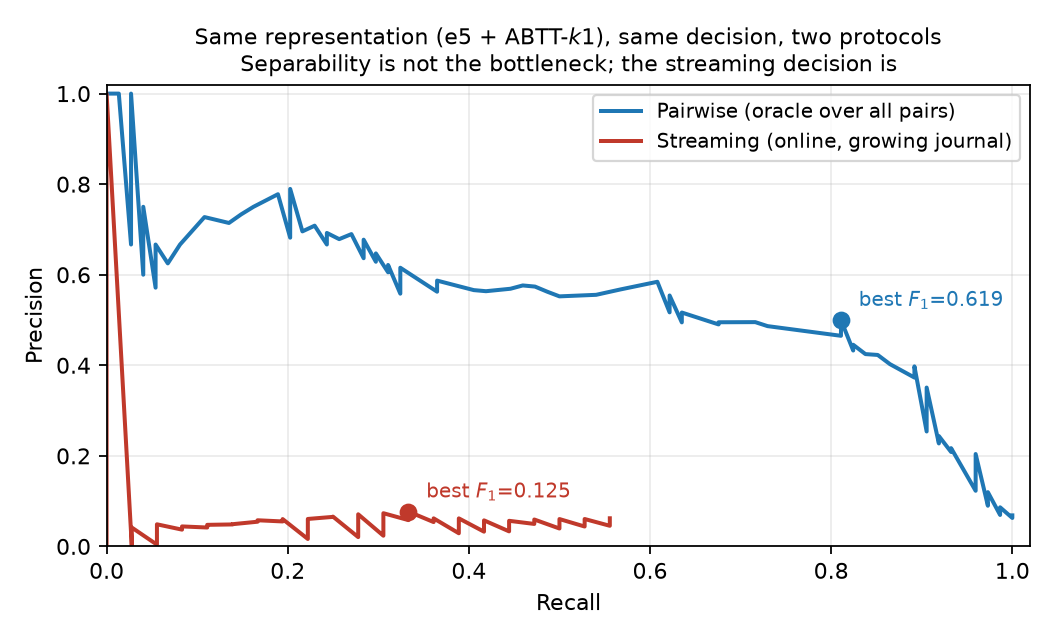
\includegraphics[width=\linewidth]{fig_gap.png}
    \caption{Precision--recall for one representation under both evaluation protocols. The
    oracle frontier sustains precision near $0.6$; the streaming frontier never exceeds
    ${\approx}0.08$. The area between them is attributable to the decision setting, not the
    embedding.}
    \label{fig:gap}
\end{figure}

\clearpage

\begin{table*}[t]
\centering\small
\begin{tabular}{p{0.30\textwidth}p{0.62\textwidth}}
\hline
\multicolumn{2}{l}{\textbf{(a) Why the decision fails: the register confound}
 \quad \emph{gold repeat event 8; e5+ABTT-$k$1 cosine}} \\
\hline
\textbf{Query} \newline 2022-12-13, Energy Ministry &
``Ministry of Energy. \emph{Request no.~177} is intended to fund 559 million shekels in
commitment authority and 4 staff positions\ldots'' \\[2pt]
\textbf{True continuation} \newline 2022-12-06 \hfill $\cos = \mathbf{0.266}$ &
``Request approved. \emph{Request no.~177}: Ministry of Energy. The request concerns the
Ministry of Energy budget line\ldots'' \\[2pt]
\textbf{Top distractor} \newline 2022-12-06, Transport \hfill $\cos = \mathbf{0.448}$ &
``\ldots they are very nice people, they smile, and they bring the request again in the same
way. Ministry of Transport\ldots'' \\
\hline
\multicolumn{2}{p{0.94\textwidth}}{\emph{The true match shares the ministry \textbf{and the
request number}; the distractor shares only bureaucratic phrasing, and still outranks it by
$0.18$. This is what the distinctiveness margin and the fingerprint extractor each attack.}}\\
\hline
\\[-6pt]
\hline
\multicolumn{2}{l}{\textbf{(b) Why log writing fails: recap-then-append}
 \quad \emph{chain ``rising milk prices'', dictalm2, zero-shot}} \\
\hline
\textbf{Entry 1} \newline 2022-11-28 (opening) &
``\ldots controlled milk prices have not changed in a decade, but input costs rose, so an
agreement was reached with the government on a moderate $4.8\%$ rise. The chair, Moshe
Gafni, asked why Israel does not subsidise dairy farmers as in Europe and the US, where
there is \textbf{no VAT on dairy}, and why \textbf{consumers must absorb the increase}
instead of the state helping the industry.'' \\[2pt]
\textbf{Entry 2} \newline 2022-11-28 (\emph{should be the increment}) &
``The chair, Moshe Gafni, stressed the need to protect dairy farmers and prevent shifting
the burden to consumers. He recalled the difference between state support elsewhere, where
\textbf{there is no VAT on dairy}, and Israel, where \textbf{consumers must absorb the
increase}. Gafni added that the dairies must not exploit the situation to raise
\emph{unregulated} prices, and that the whole chain must be handled properly.'' \\
\hline
\multicolumn{2}{p{0.94\textwidth}}{\emph{Bold marks content already present in entry~1. The
genuinely new material is one clause --- unregulated prices and the full supply chain ---
wrapped in a restatement of the previous entry. Novelty scores 18.1/100 while faithfulness
scores 80.7: the model is truthful about the record and unable to emit only the diff.}}\\
\hline
\end{tabular}
\caption{Qualitative examples behind the two central failures. Hebrew source text
translated by the authors; ellipses mark elision, emphasis added. (a) is the retrieval
confound of \cref{sec:centroid}; (b) is the novelty failure of \cref{tab:log}.}
\label{tab:examples}
\end{table*}

\clearpage

% References

\bibliography{bib}
\bibliographystyle{acl_natbib}

\end{document}
